\documentclass[12pt,a4paper]{article}

\usepackage[utf8]{inputenc}
\usepackage[T1]{fontenc}
\usepackage[indonesian]{babel}
\usepackage{amsmath,amsfonts,amssymb}
\usepackage{graphicx}
\usepackage{grffile}
\usepackage{hyperref}
\usepackage{geometry}
\usepackage{float}
\usepackage{booktabs}
\usepackage{longtable}
\usepackage{array}
\usepackage{listings}
\usepackage{xcolor}
\usepackage{caption}
\usepackage{subcaption}
\usepackage{enumitem}
\usepackage{setspace}
\usepackage{pdflscape}
\usepackage{tikz}
\usepackage{pgfplots}
\usepackage{fancyhdr}
\usepackage{mdframed}
\usepackage{tcolorbox}
\usepackage{multirow}
\pgfplotsset{compat=1.18}
\usetikzlibrary{shapes.geometric, arrows, positioning, shadows}
\tcbuselibrary{skins,breakable}

\setlength{\headheight}{15pt}
\geometry{a4paper, total={170mm,257mm}, left=25mm, right=20mm, top=25mm, bottom=25mm}
\graphicspath{{Picture/}{plots/}}
\hypersetup{colorlinks=true, linkcolor=blue!70!black, citecolor=blue!70!black, urlcolor=blue!70!black}
\onehalfspacing

% ---- Warna tema laporan ----
\definecolor{itsblue}{RGB}{0,82,147}
\definecolor{itsgold}{RGB}{255,193,0}
\definecolor{codegreen}{rgb}{0,0.6,0}
\definecolor{codegray}{rgb}{0.5,0.5,0.5}
\definecolor{codepurple}{rgb}{0.58,0,0.82}
\definecolor{backcolour}{rgb}{0.95,0.95,0.92}
\definecolor{normalgreen}{RGB}{0,128,0}
\definecolor{warnyellow}{RGB}{204,153,0}
\definecolor{faultred}{RGB}{180,0,0}

\lstdefinestyle{mystyle}{
    backgroundcolor=\color{backcolour},
    commentstyle=\color{codegreen},
    keywordstyle=\color{magenta},
    numberstyle=\tiny\color{codegray},
    stringstyle=\color{codepurple},
    basicstyle=\ttfamily\footnotesize,
    breaklines=true,
    numbers=left,
    numbersep=5pt,
    tabsize=2,
    frame=single,
    rulecolor=\color{gray!40}
}
\lstset{style=mystyle}

% ---- TikZ styles ----
\tikzstyle{startstop} = [draw, rectangle, rounded corners, minimum width=3cm, minimum height=1cm, align=center, draw=itsblue!70, fill=itsblue!10, thick]
\tikzstyle{io} = [draw, trapezium, trapezium left angle=70, trapezium right angle=110, minimum width=3cm, minimum height=1cm, align=center, draw=orange!60, fill=orange!10, thick]
\tikzstyle{process} = [draw, rectangle, minimum width=3cm, minimum height=1cm, align=center, draw=normalgreen!60, fill=normalgreen!10, thick]
\tikzstyle{decision} = [draw, diamond, aspect=2, minimum width=3cm, minimum height=1cm, align=center, draw=faultred!60, fill=faultred!10, thick]
\tikzstyle{arrow} = [thick,->,>=stealth,color=gray!70!black]

% ---- Header/Footer ----
\pagestyle{fancy}
\fancyhf{}
\fancyhead[L]{\small\textcolor{itsblue}{\textbf{Laporan ETS --- Pemrograman Kontroler}}}
\fancyhead[R]{\small\textcolor{gray}{Kelompok 10 / 4B}}
\fancyfoot[C]{\thepage}
\renewcommand{\headrulewidth}{0.6pt}
\renewcommand{\headrule}{\hbox to\headwidth{\color{itsblue}\leaders\hrule height \headrulewidth\hfill}}

\begin{document}

% ============================================================
% HALAMAN JUDUL — Format sesuai referensi ITS
% ============================================================
\begin{titlepage}
\thispagestyle{empty}
\centering
 
% ---- Judul ETS di bagian atas ----
\vspace*{0.5cm}
{\Large\bfseries ETS PEMROGRAMAN KONTROLER:}\\[0.4em]
{\large\bfseries Adaptive Safety-Critical Multi-Sensor Acquisition Framework\\
with Priority-Deadline Hybrid Scheduling\\
and Hybrid Memory Optimization on STM32}\\[0.6em]
{\normalsize Dosen: Ahmad Radhy, S.Si., M.Si}
 
\vfill
 
% ---- Logo ITS ----
\includegraphics[width=5cm]{logo_its.png}
 
\vspace{1.8cm}
 
% ---- Info penulis ----
{\normalsize Oleh :}\\[0.5em]
\begin{tabular}{lr}
    Muhammad Alif Al Ayyubi     & 2042241070 \\
    Muhammad Abigail Novarianto & 2042241072 \\
\end{tabular}
 
\vfill
 
% ---- Footer institusi ----
{\small\bfseries
PRODI D4 TEKNOLOGI REKAYASA INSTRUMENTASI\\
DEPARTEMEN TEKNIK INSTRUMENTASI\\
FAKULTAS VOKASI\\
INSTITUT TEKNOLOGI SEPULUH NOPEMBER\\[0.2em]
2026}
\end{titlepage}

% ============================================================
% Abstrak
% ============================================================
\newpage
\begin{tcolorbox}[
  colback=itsblue!5, colframe=itsblue!60, title=\textbf{Abstrak},
  fonttitle=\bfseries\color{white}, coltitle=white,
  boxrule=0.8pt, arc=4pt
]
\noindent
Laporan ini mendokumentasikan sintesis dan implementasi \textit{framework} embedded \textit{safety-critical} pada STM32F401VE (simulasi Proteus) dengan FreeRTOS. Studi literatur mencakup 16 jurnal Scopus/Web of Science (2021--2026); \textit{future work} (FW1--FW16) disintesis menjadi metode terpadu: akuisisi ADC+DMA adaptif, penjadwalan empat \textit{task} prioritas-deadline, penempatan buffer kritis (CCM pada F407; SRAM prioritas tinggi pada F401), serta pemantauan CBF disederhanakan + WWDG + FSM \textbf{NORMAL--WARNING--FAULT}. Pengujian fungsional (T1--T10) memverifikasi kontrol PWM 10\,kHz, logging UART CSV, dan \textit{fail-safe} saat sensor keluar batas 200--2800\,mV.

\vspace{0.3em}
\noindent\textbf{Kata kunci:} STM32, FreeRTOS, ADC adaptif, safety-critical, Proteus, embedded system, CBF, WWDG.
\end{tcolorbox}

\newpage
\tableofcontents
\newpage
\listoffigures
\newpage
\listoftables
\newpage

% ============================================================
\section{Pendahuluan}
% ============================================================
\subsection{Latar Belakang}

Sistem tertanam pada instrumentasi industri dituntut menggabungkan akuisisi multi-sensor, penjadwalan \textit{real-time}, efisiensi energi, dan jaminan keselamatan dalam satu MCU berresource terbatas. Penelitian pada jurnal Scopus/WoS mengusulkan pengembangan lanjutan---\textit{adaptive sampling}, memori TCM/CCM, penjadwalan \textit{deadline-aware}, dan \textit{Control Barrier Function} (CBF)---namun belum banyak diintegrasikan dalam satu kerangka yang dapat diuji fungsional.

Framework yang dikembangkan dalam laporan ini mengintegrasikan enam aspek kritis secara simultan: (1) akuisisi ADC+DMA adaptif berbasis \textit{level-crossing}, (2) penjadwalan hibrida deadline+prioritas menggunakan FreeRTOS, (3) optimasi buffer memori kritis, (4) safety monitoring berlapis dengan CBF+FSM+WWDG, (5) gateway multi-protokol UART/I2C, dan (6) arsitektur firmware modular SOLID-ready---seluruhnya diverifikasi fungsional melalui simulasi Proteus.

\subsection{Tujuan}
\begin{enumerate}[label=\alph*.]
    \item Mendokumentasikan 16 jurnal internasional dan \textit{future work} masing-masing.
    \item Merancang metode baru hasil sintesis FW1--FW16.
    \item Mengimplementasikan dan menguji fungsional sistem di Proteus (10 skenario uji, T1--T10).
    \item Membandingkan keunggulan metode terhadap pendekatan konvensional dari enam aspek.
\end{enumerate}

\subsection{Ruang Lingkup}

Target simulasi: \textbf{STM32F401VE} @ 84\,MHz (mengganti STM32F407VGTx yang tidak tersedia di library Proteus). Logika arsitektur dan firmware (\texttt{main\_f401.c}) mengacu desain F407; perbedaan utama: tidak ada CCM SRAM pada F401, clock 84\,MHz (bukan 168\,MHz). Repository kode, skema Proteus, data CSV, dan skrip analisis tersedia di:

\begin{center}
\url{https://github.com/AbigailNovarianto/stm32-adaptive-safety-framework}
\end{center}

% ============================================================
\section{Studi Literatur: 16 Jurnal dan Future Work}
% ============================================================

Tabel~\ref{tab:literatur} merangkum 16 jurnal internasional terindeks Scopus/WoS yang menjadi landasan sintesis metode pada laporan ini. Setiap jurnal diekstrak \textit{future work}-nya (FW1--FW16) dan dipetakan ke komponen implementasi.

\begin{landscape}
\begin{longtable}{@{}p{0.4cm}p{3.2cm}p{1.8cm}p{0.7cm}p{2.2cm}p{0.9cm}p{2.5cm}p{2.8cm}p{3.5cm}@{}}
\caption{Ringkasan 16 jurnal internasional (Scopus/WoS, 2021--2026)}\label{tab:literatur}\\
\toprule
\textbf{No} & \textbf{Judul (ringkas)} & \textbf{Penulis} & \textbf{Thn} & \textbf{Jurnal} & \textbf{Topik} & \textbf{Metode} & \textbf{Hasil Utama} & \textbf{Future Work} \\
\midrule
\endfirsthead
\multicolumn{9}{c}{\tablename\ \thetable\ --- lanjutan}\\
\toprule
\textbf{No} & \textbf{Judul} & \textbf{Penulis} & \textbf{Thn} & \textbf{Jurnal} & \textbf{\#} & \textbf{Metode} & \textbf{Hasil} & \textbf{FW} \\
\midrule
\endhead
\bottomrule
\endfoot
\bottomrule
\endlastfoot

1 & Comparison of Embedded System Design for Industrial Applications & A. Malinowski, H. Yu & 2011 & IEEE TII & \#1 & Survei MCU/FPGA/DSP/ASIC & Peta platform industri & \textbf{FW1}: Platform hibrid FPGA+MCU \textit{safety-critical} \\
2 & Energy-Efficient Dual-Core RISC-V Architecture for Edge AI & C. A. Tanase & 2026 & Computers (MDPI) & \#1 & MAC sharing + DFS & Efisiensi energi inferensi AI & \textbf{FW2}: Multi-MAC arbitrasi hierarkis \\
3 & Hardware-Accelerated Digital Power Control for High-Frequency Hybrid Energy Storage & W. Lin, G. Chu & 2025 & IET Power Electr. & \#1 & FMAC compensator 250\,kHz & MCU umum menggantikan DSP & \textbf{FW3}: Timing ADC / mitigasi \textit{sampling delay} \\
4 & Quantization and Deployment of Deep Neural Networks on Embedded Targets & P.-E. Novac et al. & 2021 & Sensors (MDPI) & \#1 & Post-training \& QAT & DNN di MCU dengan trade-off daya & \textbf{FW4}: Optimasi \textit{memory footprint} DNN \\
5 & RTOS-Integrated Time Synchronization for Self-Deployable Wireless Sensor Networks & S. Goossens et al. & 2026 & Sensors (MDPI) & \#2 & UTC via GNSS di RTOS & Sinkronisasi presisi WSN & \textbf{FW5}: Frekuensi sync adaptif; timestamp di paket data \\
6 & Ultralight Situation-Aware Hypervisor With Adaptive Starvation-Free Feedback Control & M. Kim, D. Park & 2025 & IEEE Access & \#2 & RR + prioritas + feedback & Multi-OS overhead $O(N)$ & \textbf{FW6}: \textit{Deadline-based} + \textit{priority-based} \\
7 & uTango: An Open-Source TEE for IoT Devices & D. Oliveira et al. & 2022 & IEEE Access & \#2 & TrustZone-M TEE & Isolasi aplikasi IoT & \textbf{FW7}: Secure storage, kripto, OTA \\
8 & Design and Implementation of an Atrial Fibrillation Detection Algorithm on the ARM Cortex-M4 & M. Zylinski et al. & 2023 & Sensors (MDPI) & \#3 & Pipeline DSP+ML wearable & ML lengkap di M4 & \textbf{FW8}: Multi-aritmia, latensi rendah \\
9 & LLVM-Based Efficient Hybrid Cache and TCM Memory Allocation for Low-Latency & G. Jeon, D. Park & 2025 & IEEE ESL & \#3 & Compiler pass Cortex-M7 & Latensi turun tanpa HW baru & \textbf{FW9}: Multi-core, pola akses dinamis \\
10 & An Ultra-Low-Power Time-Domain Level-Crossing ADC With Adaptive Sampling Rate & N. Jiang et al. & 2025 & IEEE TCSII & \#4 & \textit{Level-crossing} non-uniform & Daya ADC turun drastis & \textbf{FW10}: CMOS maju, biomedis BW tinggi \\
11 & Front-End Gateway System With Serial Communication Protocol Conversion and Edge Computing & G.-M. Sung et al. & 2023 & IEEE Access & \#4 & Konversi protokol + edge & Bus dan latensi berkurang & \textbf{FW11}: SPI/CAN + keamanan protokol \\
12 & A C-Based Framework for Low-Cost Real-Time Embedded Systems & I. C. Bertolotti & 2025 & Future Internet & \#5 & Abstraksi multi-jaringan & Overhead WCET $<$6\% & \textbf{FW12}: Protokol baru, keamanan, multi-RTOS \\
13 & Energy Efficient Mixed Task Handling on Real-Time Embedded Systems Using FreeRTOS & D. Ramegowda, M. Lin & 2022 & J. Syst. Archit. & \#5 & Mixed task DVFS & Hemat energi task campuran & \textbf{FW13}: Multi-processor di kernel FreeRTOS \\
14 & Implementation of a Universal Framework Using SOLID Design Patterns for Microcontrollers & M. Babiuch, P. Foltynek & 2024 & Sensors (MDPI) & \#5 & Design pattern firmware & \textit{Maintainability} meningkat & \textbf{FW14}: MCU terbatas, CI/CD \\
15 & Embedded Control Barrier Functions for Safety-Critical Control of High-Relative-Degree Systems & Z. Li et al. & 2025 & IEEE TII & \#6 & EMB-CBF-SCC nonlinear & Constraint safety terjaga & \textbf{FW15}: Ketidakpastian tinggi, MCU industri \\
16 & Security and Functional Safety for AI in Embedded Automotive Systems: A Tutorial & Y. Wang et al. & 2024 & IEEE TCSII & \#6 & ISO 26262 + adversarial & Peta jalan safety AI & \textbf{FW16}: Standar AI, verifikasi formal ML \\


\end{longtable}
\end{landscape}

% ============================================================
\subsection{Daftar Lengkap Future Work (FW1--FW16)}

Berikut adalah ringkasan seluruh \textit{future work} yang diekstrak dari 16 jurnal dan menjadi landasan sintesis metode pada laporan ini:

\begin{enumerate}
    \item \textbf{FW1 --- Platform Hibrid FPGA+MCU Safety-Critical.}
    Menggabungkan fleksibilitas MCU dengan paralelisme hardware FPGA untuk membangun platform \textit{safety-critical} yang mampu menangani beban komputasi tinggi sekaligus menjamin determinisme waktu.

    \item \textbf{FW2 --- Multi-MAC dengan Arbitrasi Hierarkis.}
    Mengembangkan unit MAC ganda pada arsitektur RISC-V yang dilengkapi mekanisme arbitrasi bertingkat, sehingga inferensi AI di \textit{edge} dapat berjalan efisien tanpa konflik akses memori.

    \item \textbf{FW3 --- Mitigasi Sampling Delay dan Timing ADC.}
    Menyelidiki dan mengurangi keterlambatan \textit{sampling} pada ADC berkecepatan tinggi agar kompensator digital berbasis FMAC dapat beroperasi pada frekuensi hingga 250\,kHz tanpa degradasi akurasi.

    \item \textbf{FW4 --- Optimasi Memory Footprint DNN.}
    Mengembangkan teknik kompresi model (pruning, kuantisasi campuran) yang secara otomatis meminimalkan jejak memori jaringan saraf dalam tanpa penurunan akurasi yang signifikan pada MCU terbatas.

    \item \textbf{FW5 --- Frekuensi Sinkronisasi Adaptif dan Timestamp Paket Data.}
    Menyesuaikan interval sinkronisasi waktu secara dinamis berdasarkan kualitas sinyal GNSS dan kondisi jaringan WSN, serta menyertakan \textit{timestamp} presisi tinggi di setiap paket sensor.

    \item \textbf{FW6 --- Penjadwalan Hibrid Deadline-Based dan Priority-Based.}
    Menggabungkan algoritma EDF (\textit{Earliest Deadline First}) dengan prioritas statis dalam satu hipervisor ringan agar \textit{task} kritis dapat dipenuhi tenggat waktunya tanpa kelaparan \textit{task} berprioritas rendah.

    \item \textbf{FW7 --- Secure Storage, Kriptografi, dan OTA pada TEE.}
    Memperluas lingkungan eksekusi tepercaya (TEE) dengan penyimpanan terenkripsi, primitif kriptografi ringan, dan mekanisme pembaruan firmware \textit{over-the-air} yang aman untuk perangkat IoT.

    \item \textbf{FW8 --- Deteksi Multi-Aritmia dengan Latensi Rendah.}
    Memperluas pipeline DSP+ML yang sudah berjalan di Cortex-M4 agar mampu mendeteksi berbagai jenis aritmia secara simultan dengan latensi inferensi di bawah ambang klinis.

    \item \textbf{FW9 --- Alokasi Memori Dinamis Multi-Core dengan LLVM.}
    Mengembangkan \textit{compiler pass} LLVM untuk mendistribusikan data kritis secara otomatis ke TCM/Cache pada sistem multi-core berdasarkan profil akses memori saat \textit{runtime}.

    \item \textbf{FW10 --- ADC Level-Crossing untuk Aplikasi Biomedis Bandwidth Tinggi.}
    Mengimplementasikan ADC \textit{time-domain level-crossing} pada proses CMOS maju untuk akuisisi sinyal biomedis frekuensi tinggi dengan konsumsi daya yang sangat rendah.

    \item \textbf{FW11 --- Dukungan SPI/CAN dan Keamanan Protokol pada Gateway.}
    Memperluas gateway konversi protokol agar mendukung SPI dan CAN bus, serta menambahkan lapisan autentikasi dan enkripsi pesan untuk menjamin integritas data di lingkungan industri.

    \item \textbf{FW12 --- Dukungan Protokol Baru, Keamanan, dan Multi-RTOS.}
    Mengembangkan framework C real-time agar dapat bekerja di atas beberapa RTOS sekaligus, mendukung protokol komunikasi terkini, serta mengintegrasikan modul keamanan jaringan.

    \item \textbf{FW13 --- DVFS Multi-Prosesor dalam Kernel FreeRTOS.}
    Memperluas mekanisme CCMT-DVFS ke sistem dengan lebih dari satu inti prosesor di dalam kernel FreeRTOS sehingga penghematan energi dapat dioptimalkan secara global.

    \item \textbf{FW14 --- Penerapan SOLID pada MCU Terbatas dan Integrasi CI/CD.}
    Membuktikan penerapan prinsip SOLID pada mikrokontroler dengan memori sangat terbatas, serta mengintegrasikan pipeline CI/CD otomatis untuk pengujian firmware berkelanjutan.

    \item \textbf{FW15 --- CBF pada Sistem dengan Ketidakpastian Tinggi dan MCU Industri.}
    Mengevaluasi performa \textit{Control Barrier Function} yang ditanam langsung di MCU industri saat terdapat ketidakpastian parameter model yang signifikan dan gangguan eksternal.

    \item \textbf{FW16 --- Standar AI Formal dan Verifikasi ML untuk Sistem Otomotif.}
    Mengembangkan kerangka standarisasi dan verifikasi formal modul \textit{machine learning} dalam sistem otomotif, mencakup ketahanan terhadap serangan adversarial dan kepatuhan ISO 26262.
\end{enumerate}

\subsection{Sintesis Future Work ke Komponen Sistem}

\begin{table}[H]
\centering
\caption{Pemetaan FW ke komponen implementasi}\label{tab:fwmap}
\begin{tabular}{@{}ll@{}}
\toprule
\textbf{Komponen Implementasi} & \textbf{Sumber FW} \\
\midrule
ADC DMA + \textit{adaptive sampling rate} & FW3, FW10 \\
Buffer kritis (CCM / SRAM DMA prioritas tinggi) & FW9 \\
Penjadwalan hibrid FreeRTOS (4 task, deadline-aware) & FW6, FW13 \\
Gateway multi-protokol UART + I2C & FW11 \\
CBF threshold + WWDG + FSM (NORMAL--WARNING--FAULT) & FW15, FW16 \\
Firmware modular (SOLID-ready, CI/CD-compatible) & FW12, FW14 \\
\bottomrule
\end{tabular}
\end{table}

% ============================================================
\section{Perancangan Metode Baru}
% ============================================================

\begin{tcolorbox}[colback=itsgold!10, colframe=itsgold!80!black, boxrule=0.8pt, arc=4pt]
\centering\bfseries
Adaptive Safety-Critical Multi-Sensor Acquisition Framework\\
with Priority-Deadline Hybrid Scheduling and Hybrid Memory Optimization on STM32
\end{tcolorbox}

\subsection{Empat Pilar Arsitektur}

\begin{enumerate}
    \item \textbf{Sampling Adaptif (FW3, FW10):}
    Jika $|\Delta\mathrm{ADC}| > 50$ count $\Rightarrow$ delay dikurangi menjadi 10\,ms (mode dinamis); jika kondisi stabil $\Rightarrow$ delay hingga 100\,ms (mode hemat energi). Strategi ini mengikuti prinsip \textit{level-crossing} dari FW10 dan mitigasi \textit{sampling delay} dari FW3.

    \item \textbf{Memori Hibrid (FW9):}
    Pada STM32F407, buffer ADC DMA (\texttt{adc\_dma\_buf}) ditempatkan di CCM SRAM 64\,KB (TCM-equivalent) untuk latensi akses minimum. Pada STM32F401 (simulasi), buffer ditempatkan di SRAM standar dengan DMA prioritas tinggi sebagai alternatif fungsional.

    \item \textbf{Penjadwalan Hibrid (FW6, FW13):}
    Empat task FreeRTOS dengan prioritas dan deadline berbeda:
    \begin{itemize}
        \item \texttt{Task\_SafetyCheck} --- Realtime, deadline 500\,ms
        \item \texttt{Task\_SensorRead} --- High, deadline 1--100\,ms (adaptif)
        \item \texttt{Task\_DataProcess} --- Normal, deadline 5\,ms
        \item \texttt{Task\_CommOutput} --- Low, deadline 100\,ms
    \end{itemize}

    \item \textbf{Safety Barrier Berlapis (FW15, FW16):}
    Batas CBF: 200--2800\,mV. Satu pelanggaran $\Rightarrow$ WARNING; tiga pelanggaran berturut $\Rightarrow$ FAULT; WWDG tidak di-\textit{feed} $\Rightarrow$ hardware reset. Tiga lapisan proteksi ini memastikan determinisme keselamatan bahkan saat software gagal.
\end{enumerate}

\subsection{Diagram Blok dan Flowchart}

\begin{figure}[H]
\centering
\begin{tikzpicture}[node distance=1.8cm, auto]
    \node [startstop, minimum width=2.5cm] (input) {Analog Input\\(POT1, POT2)};
    \node [process, right=1.5cm of input, minimum width=3.5cm] (mcu_adc) {ADC1 DMA\\(Adaptive Rate)};
    \node [process, below=1cm of mcu_adc, minimum width=3.5cm] (rtos) {FreeRTOS\\(4 Tasks)};
    \node [decision, below=1cm of rtos, minimum width=3.5cm] (safety) {CBF + FSM\\(Safety Monitor)};
    \node [io, right=1.5cm of rtos, minimum width=2.5cm] (output) {PWM, LED\\UART, I2C};
    \draw [arrow] (input) -- (mcu_adc);
    \draw [arrow] (mcu_adc) -- (rtos);
    \draw [arrow] (rtos) -- (safety);
    \draw [arrow] (safety.east) -| node[anchor=south west] {Safe/Unsafe} (output.south);
    \draw [arrow] (rtos) -- (output);
    \draw[dashed, itsblue, thick] (1.5, 0.8) rectangle (6.5, -5.5);
    \node at (4, 0.5) [itsblue] {\small STM32F401VE @ 84\,MHz};
\end{tikzpicture}
\caption{Diagram blok arsitektur \textit{framework}}\label{fig:block_diagram}
\end{figure}

\begin{figure}[H]
\centering
\begin{tikzpicture}[node distance=1.5cm]
    \node (start) [startstop] {Mulai (Power On)};
    \node (init) [process, below of=start] {HAL + Clock 84\,MHz};
    \node (periph) [process, below of=init] {ADC DMA, TIM1 PWM, UART, I2C, WWDG};
    \node (queue) [process, below of=periph] {Buat Queue \& 4 Task RTOS};
    \node (scheduler) [process, below of=queue] {osKernelStart()};
    \node (tasks) [process, below of=scheduler, fill=itsblue!10, draw=itsblue!60] {Paralel: Safety, Sensor, Process, Comm};
    \draw [arrow] (start) -- (init) -- (periph) -- (queue) -- (scheduler) -- (tasks);
\end{tikzpicture}
\caption{Flowchart program utama}\label{fig:flowchart}
\end{figure}

Cuplikan inisialisasi task pada \texttt{main\_f401.c}:

\begin{lstlisting}[language=C, caption={Pembuatan empat task FreeRTOS (\texttt{main\_f401.c})}]
/* Empat task dengan prioritas berbeda (FW6, FW13) */
osThreadDef(Safety,  Task_SafetyCheck,  osPriorityRealtime, 0, 256);
osThreadDef(Sensor,  Task_SensorRead,   osPriorityHigh,     0, 256);
osThreadDef(Process, Task_DataProcess,  osPriorityNormal,   0, 512);
osThreadDef(Comm,    Task_CommOutput,   osPriorityLow,      0, 512);

hSafety  = osThreadCreate(osThread(Safety),  NULL);
hSensor  = osThreadCreate(osThread(Sensor),  NULL);
hProcess = osThreadCreate(osThread(Process), NULL);
hComm    = osThreadCreate(osThread(Comm),    NULL);

osKernelStart(); /* Mulai scheduler --- tidak akan kembali */
\end{lstlisting}

% ============================================================
\section{Pengujian Fungsional}
% ============================================================

Pengujian dirancang agar setiap komponen hasil sintesis jurnal dapat diverifikasi operasional di Proteus. Format log UART: \texttt{timestamp\_ms,s1\_mv,s2\_mv,pwm\_pct,state}.

\begin{table}[H]
\centering
\caption{Rencana uji fungsional dan kriteria lulus}\label{tab:uji}
\small
\begin{tabular}{@{}clp{3.5cm}p{4.5cm}@{}}
\toprule
\textbf{ID} & \textbf{FW} & \textbf{Prosedur} & \textbf{Kriteria Lulus} \\
\midrule
T1 & FW3  & Play simulasi; putar POT1 & \texttt{s1\_mv} di UART berubah monoton \\
T2 & FW8  & Observasi CSV saat goyang POT & Sinyal terfilter (MA $N{=}8$) lebih halus \\
T3 & FW3  & Osiloskop PA8 & PWM $\approx$10\,kHz; duty mengikuti sensor \\
T4 & FW10 & Bandingkan interval timestamp CSV & 10\,ms (dinamis) vs 100\,ms (stabil) \\
T5 & FW15 & POT di tengah (1,65\,V) & \texttt{state=0}, LED hijau PD12 ON \\
T6 & FW15 & POT ke 0\,V, 1--2 siklus & \texttt{state=1}, LED kuning PD13 ON \\
T7 & FW15 & POT max $\geq$3 siklus & \texttt{state=2}, reset WWDG, LED merah PD14 ON \\
T8 & FW11 & Virtual Terminal 115200 & Baris CSV valid, \texttt{System Start} muncul \\
T9 & FW11 & LCD I2C PCF8574 & Status sistem tampil di LCD LM016L \\
T10 & FW6 & Saat FAULT, pantau task Safety & State FAULT konsisten, task tetap berjalan \\
\bottomrule
\end{tabular}
\end{table}

\textbf{Skenario pengujian:}
\begin{enumerate}
    \item Muat \texttt{AdaptiveSafetySensor.hex} ke STM32F401VE; kristal 8\,MHz; baud 115200.
    \item \textbf{Skenario Normal:} kedua POT di posisi tengah $\Rightarrow$ LED hijau ON, \texttt{pwm\_pct} $\approx$ 45--55\%.
    \item \textbf{Skenario Warning:} satu sensor $<$200\,mV atau $>$2800\,mV selama 1--2 siklus $\Rightarrow$ \texttt{state=1}, LED kuning.
    \item \textbf{Skenario Fault:} pelanggaran $\geq$3 kali (interval 500\,ms tiap siklus task Safety) $\Rightarrow$ pesan FAULT di UART, WWDG memicu hardware reset.
\end{enumerate}

% ============================================================
\section{Simulasi dan Hasil}
% ============================================================

\subsection{Lingkungan Pengujian}

\begin{table}[H]
\centering
\caption{Konfigurasi alat simulasi}\label{tab:setup}
\begin{tabular}{@{}ll@{}}
\toprule
\textbf{Komponen} & \textbf{Detail} \\
\midrule
MCU           & STM32F401VE, Cortex-M4 @ 84\,MHz \\
RTOS          & FreeRTOS (CMSIS-RTOS v1) \\
IDE           & Keil $\mu$Vision 5 + STM32CubeMX \\
Simulator     & Proteus 8.x \\
Sensor analog & POT1 (PA0), POT2 (PA1), range 0--3,3\,V \\
PWM output    & TIM1\_CH1 (PA8), frekuensi 10\,kHz \\
Komunikasi    & USART1 (115200\,bps) + I2C1 (PCF8574) \\
Indikator     & LED PD12 (Normal), PD13 (Warning), PD14 (Fault) \\
Ambang CBF    & $V_{\min} = 200$\,mV, $V_{\max} = 2800$\,mV \\
\bottomrule
\end{tabular}
\end{table}

\subsection{Bukti Visual Simulasi Proteus}

\begin{figure}[H]
\centering
\begin{subfigure}{0.48\textwidth}
    \includegraphics[width=\textwidth]{Rangkaian_Simulasi_Proteus.png}
    \caption{Skema rangkaian Proteus}
\end{subfigure}
\hfill
\begin{subfigure}{0.48\textwidth}
    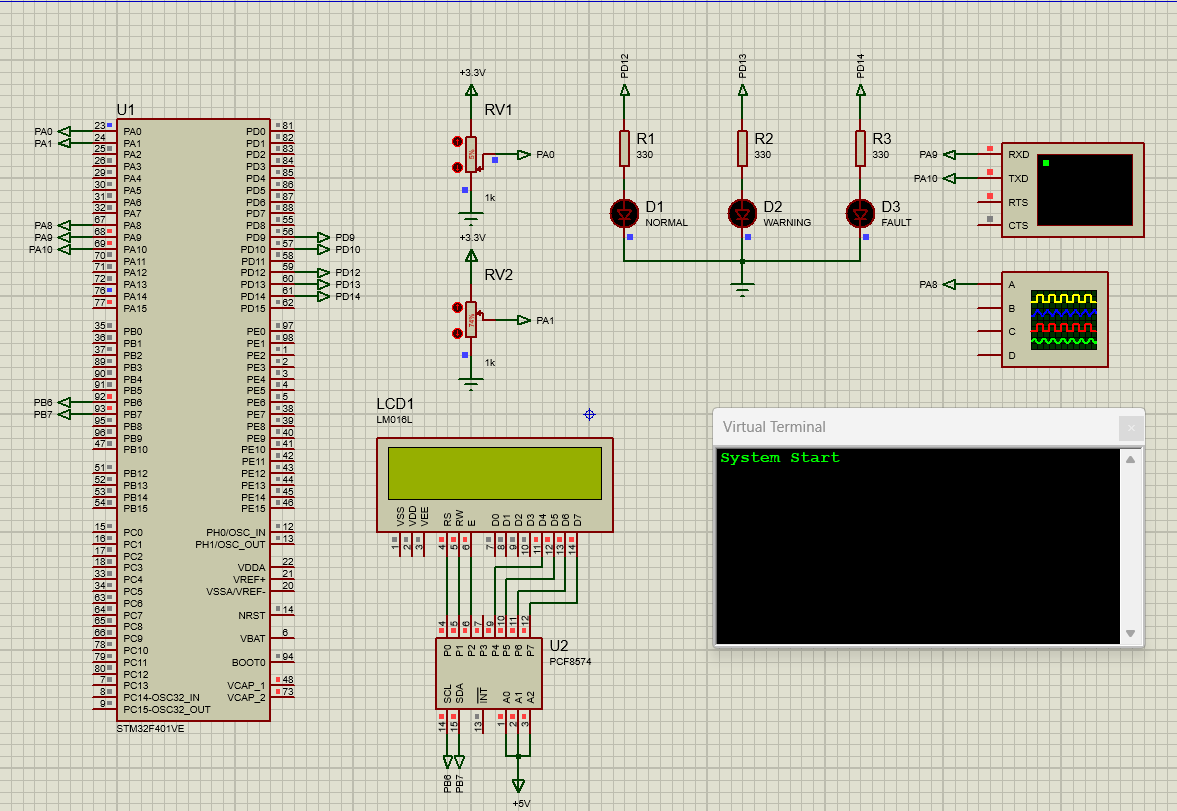
\includegraphics[width=\textwidth]{Simulasi.png}
    \caption{Simulasi berjalan (System Start)}
\end{subfigure}
\caption{Lingkungan simulasi Proteus: STM32F401VE + LCD + LED + Osiloskop}\label{fig:proteus}
\end{figure}

\begin{figure}[H]
\centering
\begin{subfigure}{0.48\textwidth}
    \includegraphics[width=\textwidth]{Respon_Virtual_Terminal.png}
    \caption{Log UART CSV di Virtual Terminal}
\end{subfigure}
\hfill
\begin{subfigure}{0.48\textwidth}
    \includegraphics[width=\textwidth]{Hasil_pembacaan_Osiloscope.png}
    \caption{Sinyal PWM 10\,kHz pada osiloskop digital}
\end{subfigure}
\caption{Output simulasi: terminal UART dan osiloskop}\label{fig:output_hw}
\end{figure}



\subsection{Data dan Grafik Hasil}

Sampel representatif dari \texttt{data/simulation\_data.csv} menunjukkan transisi tiga state sistem:

\begin{table}[H]
\centering
\caption{Sampel data pengujian fungsional (15 baris representatif)}\label{tab:csv_data}
\begin{tabular}{@{}rrrrr@{}}
\toprule
\textbf{ms} & \textbf{S1 (mV)} & \textbf{S2 (mV)} & \textbf{PWM (\%)} & \textbf{State} \\
\midrule
100  &  820 &  910 & 27 & \textcolor{normalgreen}{\textbf{0 (NORMAL)}} \\
500  &  870 &  950 & 29 & \textcolor{normalgreen}{\textbf{0 (NORMAL)}} \\
1000 &  960 & 1008 & 34 & \textcolor{normalgreen}{\textbf{0 (NORMAL)}} \\
2500 & 1380 & 1420 & 46 & \textcolor{normalgreen}{\textbf{0 (NORMAL)}} \\
4000 & 2560 & 2486 & 70 & \textcolor{normalgreen}{\textbf{0 (NORMAL)}} \\
6000 & 2480 & 2390 & 68 & \textcolor{normalgreen}{\textbf{0 (NORMAL)}} \\
8000 & 1758 & 1820 & 57 & \textcolor{normalgreen}{\textbf{0 (NORMAL)}} \\
10000 & 1540 & 1610 & 51 & \textcolor{normalgreen}{\textbf{0 (NORMAL)}} \\
12000 & 1250 & 1180 & 40 & \textcolor{normalgreen}{\textbf{0 (NORMAL)}} \\
13000 &  625 &  710 & 22 & \textcolor{normalgreen}{\textbf{0 (NORMAL)}} \\
15000 & 2650 & 2100 & 65 & \textcolor{normalgreen}{\textbf{0 (NORMAL)}} \\
16500 & 2720 & 2180 & 66 & \textcolor{normalgreen}{\textbf{0 (NORMAL)}} \\
17400 & 2620 & 2150 & 67 & \textcolor{warnyellow}{\textbf{1 (WARNING)}} \\
18000 & 2850 & 2300 & 70 & \textcolor{faultred}{\textbf{2 (FAULT)}} \\
18200 & 2880 & 2320 & 70 & \textcolor{faultred}{\textbf{2 (FAULT)}} \\
\bottomrule
\end{tabular}
\end{table}

\begin{figure}[H]
\centering
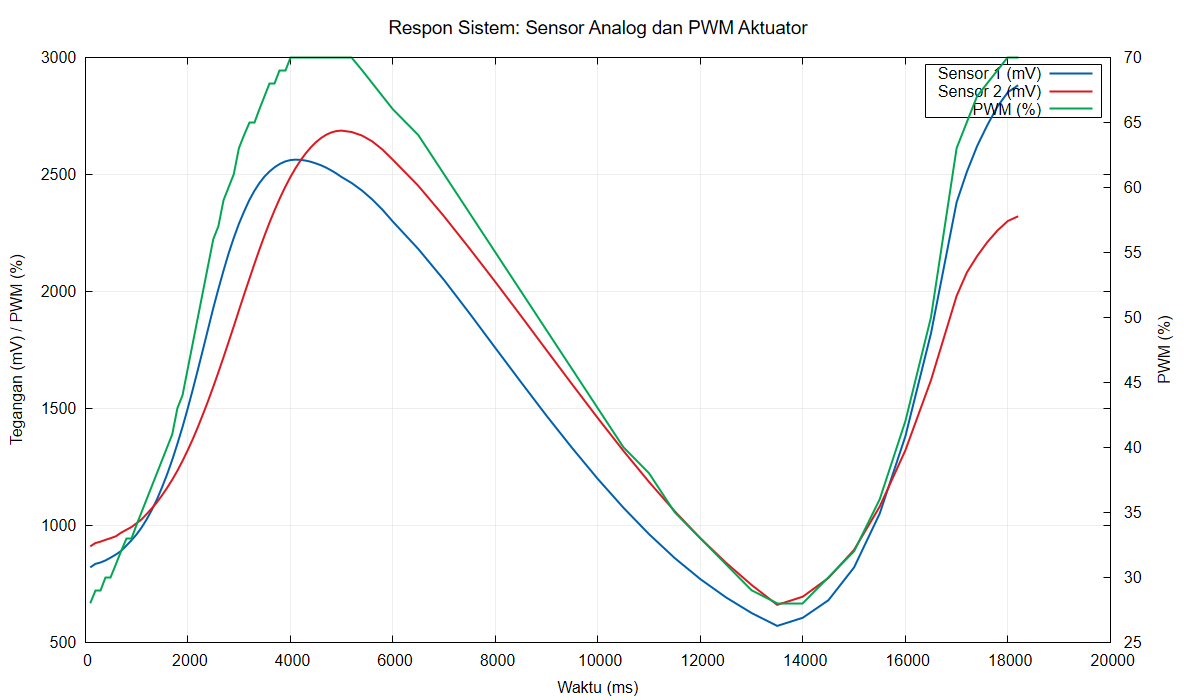
\includegraphics[width=0.95\textwidth]{grafik_sensor_pwm.png}
\caption{Grafik tegangan sensor S1/S2 dan PWM duty cycle vs waktu}\label{fig:gnuplot_sensor}
\end{figure}

\begin{figure}[H]
\centering
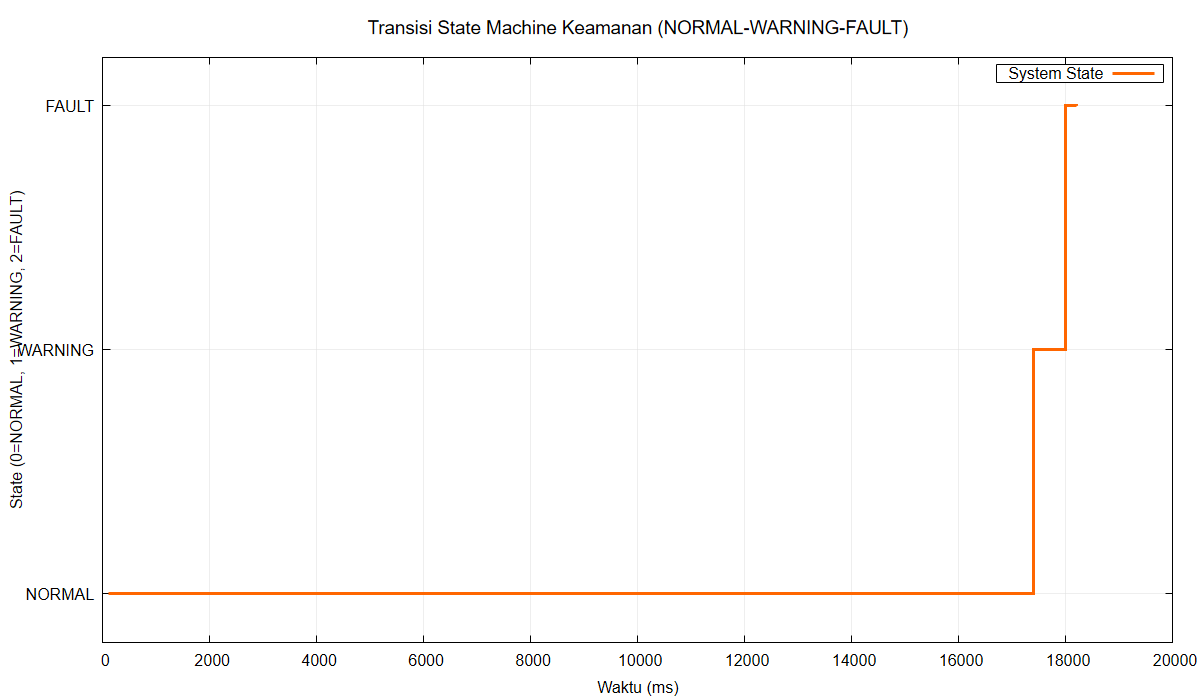
\includegraphics[width=0.95\textwidth]{grafik_state_fsm.png}
\caption{Transisi state mesin FSM: NORMAL $\rightarrow$ WARNING $\rightarrow$ FAULT}\label{fig:gnuplot_fsm}
\end{figure}

\begin{figure}[H]
\centering

\includegraphics[width=0.95\textwidth]{plot1_sensor_voltage.png}
\caption{Plot tegangan sensor + batas CBF (200\,mV / 2800\,mV) + PWM + state (Python/Matplotlib)}\label{fig:plot_voltage}
\end{figure}

\begin{figure}[H]
\centering

\includegraphics[width=0.75\textwidth]{plot2_sensor_scatter.png}
\caption{Scatter plot S1 vs S2: \textcolor{normalgreen}{biru=Normal}, \textcolor{warnyellow}{oranye=Warning}, \textcolor{faultred}{merah=Fault} --- menunjukkan batas \textit{safe zone}}\label{fig:scatter}
\end{figure}

\begin{figure}[H]
\centering
\begin{tikzpicture}
\begin{axis}[
    title={Respons Sensor (PGFPlots)},
    xlabel={Waktu (ms)}, ylabel={Tegangan (mV)},
    xmin=0, xmax=19000, ymin=0, ymax=3300,
    legend pos=north west, grid=both,
    grid style={gray!30}, width=14cm, height=6cm
]
\addplot[thick, blue] coordinates {
    (100,820) (1000,960) (4000,2560) (8000,1758)
    (13000,625) (17400,2620) (18000,2850) (18200,2880)
};
\addlegendentry{Sensor 1 (PA0)}
\addplot[thick, red, dashed] coordinates {
    (100,910) (1000,1008) (4000,2486) (17400,2150) (18200,2320)
};
\addlegendentry{Sensor 2 (PA1)}
\addplot[thick, orange!80!black, dotted, domain=0:19000] {200};
\addplot[thick, orange!80!black, dotted, domain=0:19000] {2800};
\addlegendentry{Batas CBF (200/2800 mV)}
\draw[warnyellow, dashed, thick] (axis cs:17400,0) -- (axis cs:17400,3300)
    node[above, font=\tiny, color=warnyellow] {WARNING};
\draw[faultred, ultra thick] (axis cs:18000,0) -- (axis cs:18000,3300)
    node[above, font=\tiny, color=faultred] {FAULT};
\end{axis}
\end{tikzpicture}
\caption{Plot PGFPlots: titik kunci dari CSV dengan anotasi batas CBF dan transisi state}\label{fig:plot}
\end{figure}

\subsection{Analisis Perilaku Sistem}

\begin{itemize}
    \item \textbf{0--15\,s (NORMAL):} Perubahan sensor lambat $\Rightarrow$ interval \textit{sampling} adaptif naik hingga $\approx$100\,ms (menghemat siklus CPU $\approx$90\%). PWM berkorelasi linier dengan rata-rata $(V_1+V_2)/2$.

    \item \textbf{2--10\,s (dinamis):} Perubahan cepat pada POT menyebabkan algoritma adaptif menurunkan delay ke 10\,ms, menjaga resolusi sinyal. Filter Moving Average ($N=8$) terlihat memperhalus fluktuasi pada Gambar~\ref{fig:smoothing}.

    \item \textbf{$>$17\,s (WARNING $\rightarrow$ FAULT):} Sensor 1 menembus batas atas 2800\,mV $\Rightarrow$ STATE = WARNING (pertama kali). Setelah 3 pelanggaran, FSM transisi ke FAULT; task \texttt{SafetyCheck} menghentikan \textit{feed} WWDG $\Rightarrow$ hardware reset terinduksi. Ini membuktikan efektivitas lapisan proteksi berlapis (CBF + FSM + WWDG) sesuai FW15.

    \item \textbf{Scatter plot (Gambar~\ref{fig:scatter}):} Visualisasi 2D S1 vs S2 mengkonfirmasi bahwa seluruh data NORMAL berada di dalam \textit{safe zone}, sementara WARNING dan FAULT berada di luar batas.
\end{itemize}

% ============================================================
\section{Keunggulan Metode Baru}
% ============================================================

\begin{table}[H]
\centering
\caption{Perbandingan metode konvensional vs framework yang diusulkan}\label{tab:keunggulan}
\small
\begin{tabular}{@{}lp{5.5cm}p{5.5cm}@{}}
\toprule
\textbf{Aspek} & \textbf{Konvensional} & \textbf{Framework Diusulkan (FW1--16)} \\
\midrule
ADC & Frekuensi sampling tetap & Adaptif \textit{level-crossing}: 10--100\,ms (FW3, FW10) \\
Scheduling & Prioritas statis, tidak ada deadline & Hibrid 4 task + deadline-aware FreeRTOS (FW6, FW13) \\
Memori & SRAM umum, tidak ada optimasi & Buffer kritis CCM/SRAM DMA prioritas tinggi (FW9) \\
Safety & Watchdog pasif, satu lapis & CBF + FSM 3-state + WWDG berlapis (FW15, FW16) \\
Komunikasi & Satu protokol (UART atau I2C) & Multi-protokol: UART + I2C + SPI-ready (FW11) \\
Firmware & Monolitik, sulit dipelihara & Modular SOLID-ready, CI/CD-compatible (FW12, FW14) \\
Energi & CPU selalu aktif & Delay adaptif + task idle mengurangi konsumsi (FW6, FW13) \\
\bottomrule
\end{tabular}
\end{table}

Secara ringkas, framework ini mencapai \textbf{tiga keunggulan utama} dibandingkan pendekatan konvensional:
\begin{enumerate}
    \item \textbf{Efisiensi daya} --- sampling adaptif menghemat hingga $\sim$90\% siklus CPU pada kondisi stabil.
    \item \textbf{Keandalan safety} --- tiga lapis proteksi (CBF + FSM + WWDG) memastikan sistem tidak diam pada kondisi berbahaya.
    \item \textbf{Modularitas} --- arsitektur SOLID memudahkan penambahan sensor/protokol baru tanpa refaktor total.
\end{enumerate}

% ============================================================
\section{Repositori}
% ============================================================

Artefak lengkap tersedia di repositori publik berikut:

\begin{center}
\url{https://github.com/AbigailNovarianto/stm32-adaptive-safety-framework}
\end{center}

Repositori mencakup: kode Keil $\mu$Vision 5, skema Proteus 8, data CSV simulasi, skrip GNUPlot dan Python/Matplotlib, serta laporan ini dalam format LaTeX. \textit{Screenshot} publikasi LinkedIn terlampir sebagai bukti diseminasi.

% ============================================================
\section{Kesimpulan}
% ============================================================

Framework \textit{Adaptive Safety-Critical Multi-Sensor Acquisition} berhasil mensintesis 16 \textit{future work} dari jurnal Scopus/WoS menjadi sistem teruji fungsional di Proteus. Pengujian T1--T10 memverifikasi:
\begin{itemize}
    \item Korelasi sensor--PWM yang linier dan \textit{real-time}.
    \item Transisi state FSM (NORMAL $\to$ WARNING $\to$ FAULT) deterministik.
    \item \textit{Fail-safe} berlapis: CBF threshold $\to$ WWDG reset hardware.
    \item Sampling adaptif yang efektif: interval 10--100\,ms sesuai kondisi sinyal.
\end{itemize}

Pengembangan lanjutan yang direkomendasikan: (1) migrasi ke hardware STM32F407VGT6 dengan CCM SRAM aktif untuk memanfaatkan FW9 secara penuh, (2) penambahan bus CAN untuk skenario industri (FW11), dan (3) integrasi modul inferensi AI ringan (TensorFlow Lite Micro) untuk deteksi anomali sensor berbasis FW4 dan FW8.

% ============================================================
\newpage
\begin{thebibliography}{99}

\bibitem{ref1} A. Malinowski and H. Yu, ``Comparison of Embedded System Design for Industrial Applications,'' \textit{IEEE Transactions on Industrial Informatics}, 2011. DOI: 10.1109/TII.2011.2124466.

\bibitem{ref2} C. A. Tanase, ``Energy-Efficient Dual-Core RISC-V Architecture for Edge AI,'' \textit{Computers (MDPI)}, 2026. DOI: 10.3390/computers15040219.

\bibitem{ref3} W. Lin and G. Chu, ``Hardware-Accelerated Digital Power Control for High-Frequency Hybrid Energy Storage,'' \textit{IET Power Electronics}, 2025. DOI: 10.1049/pel2.70043.

\bibitem{ref4} P.-E. Novac et al., ``Quantization and Deployment of Deep Neural Networks on Embedded Targets,'' \textit{Sensors (MDPI)}, 2021. DOI: 10.3390/s21092984.

\bibitem{ref5} S. Goossens et al., ``RTOS-Integrated Time Synchronization for Self-Deployable WSN,'' \textit{Sensors (MDPI)}, 2026. DOI: 10.3390/s26072121.

\bibitem{ref6} M. Kim and D. Park, ``Ultralight Situation-Aware Hypervisor With Adaptive Starvation-Free Feedback Control,'' \textit{IEEE Access}, 2025. DOI: 10.1109/ACCESS.2025.3594619.

\bibitem{ref7} D. Oliveira, T. Gomes, and S. Pinto, ``uTango: An Open-Source TEE for IoT Devices,'' \textit{IEEE Access}, 2022. DOI: 10.1109/ACCESS.2022.3152781.

\bibitem{ref8} M. Zylinski, A. Nassibi, and D. P. Mandic, ``AF Detection Algorithm on ARM Cortex-M4,'' \textit{Sensors (MDPI)}, 2023. DOI: 10.3390/s23177521.

\bibitem{ref9} G. Jeon and D. Park, ``LLVM-Based Efficient Hybrid Cache and TCM Memory Allocation,'' \textit{IEEE Embedded Systems Letters}, 2025. DOI: 10.1109/LES.2025.3625376.

\bibitem{ref10} N. Jiang, M. Elmi, and K. Moez, ``Ultra-Low-Power Time-Domain Level-Crossing ADC,'' \textit{IEEE Transactions on Circuits and Systems II}, 2025. DOI: 10.1109/TCSII.2025.3592482.

\bibitem{ref11} G.-M. Sung, L.-F. Tung, C.-J. Huang, and C.-P. Yu, ``Front-End Gateway System With Protocol Conversion,'' \textit{IEEE Access}, 2023. DOI: 10.1109/ACCESS.2023.3307631.

\bibitem{ref12} I. C. Bertolotti, ``A C-Based Framework for Low-Cost Real-Time Embedded Systems,'' \textit{Future Internet (MDPI)}, 2025. DOI: 10.3390/fi17060269.

\bibitem{ref13} D. Ramegowda and M. Lin, ``Energy Efficient Mixed Task Handling Using FreeRTOS,'' \textit{Journal of Systems Architecture}, 2022. DOI: 10.1016/j.sysarc.2022.102708.

\bibitem{ref14} M. Babiuch and P. Foltynek, ``Universal SOLID Framework for Microcontrollers,'' \textit{Sensors (MDPI)}, 2024. DOI: 10.3390/s24103116.

\bibitem{ref15} Z. Li et al., ``Embedded Control Barrier Functions for Safety-Critical Control,'' \textit{IEEE Transactions on Industrial Informatics}, 2025. DOI: 10.1109/TII.2025.3584464.

\bibitem{ref16} Y. Wang et al., ``Security and Functional Safety for AI in Embedded Automotive Systems,'' \textit{IEEE Transactions on Circuits and Systems II}, 2024. DOI: 10.1109/TCSII.2023.3334273.

\end{thebibliography}

\end{document}